\documentclass[10pt,twocolumn,letterpaper]{article}
\usepackage[rebuttal]{cvpr}

% Include other packages here, before hyperref.
\usepackage{graphicx}
\usepackage{amsmath}
\usepackage{amssymb}
\usepackage{booktabs}
\usepackage[dvipsnames]{xcolor}

% \newcommand{\red}[1]{\textcolor{red}{#1}}
% \newcommand{\blue}[1]{\textcolor{blue}{#1}}
% Import additional packages in the preamble file, before hyperref
\input{preamble}

% If you comment hyperref and then uncomment it, you should delete
% egpaper.aux before re-running latex.  (Or just hit 'q' on the first latex
% run, let it finish, and you should be clear).
\definecolor{cvprblue}{rgb}{0.21,0.49,0.74}
\usepackage[pagebackref,breaklinks,colorlinks,allcolors=cvprblue]{hyperref}

% If you wish to avoid re-using figure, table, and equation numbers from
% the main paper, please uncomment the following and change the numbers
% appropriately.
%\setcounter{figure}{2}
%\setcounter{table}{1}
%\setcounter{equation}{2}

% If you wish to avoid re-using reference numbers from the main paper,
% please uncomment the following and change the counter value to the
% number of references you have in the main paper (here, 100).
%\makeatletter
%\apptocmd{\thebibliography}{\global\c@NAT@ctr 100\relax}{}{}
%\makeatother

%%%%%%%%% PAPER ID  - PLEASE UPDATE
\def\paperID{N/A} % *** Enter the Paper ID here
\def\confName{CVPR}
\def\confYear{2026}

\begin{document}

%%%%%%%%% TITLE - PLEASE UPDATE
\title{Bridge: Basis-Driven Causal Inference Marries VFMs for Domain Generalization}  % **** Enter the paper title here

\maketitle
\thispagestyle{empty}
\appendix

We thank all the reviewers' constructive feedback and positive comments, 
\textit{e.g.}, ``clear strengths'' (\textcolor{red}{aZkC}), 
``novel technical framework'' (\textcolor{blue}{C8PF}), 
and ``strong and comprehensive experimental results'' (\textcolor{orange}{qwmm}, \textcolor{blue}{C8PF}, \textcolor{red}{aZkC}). 
The discussion outcomes will be merged into the revised version.


\noindent\textbf{\textcolor{blue}{C8PF}: Eq. (3) $\to$ (4).}
% Many thanks for pointing this out.
Following FSCI [35] and DIC [82], we employ the Normalized Weighted Geometric Mean (NWGM) to approximate Eq. (3) as:
% Following FSCI (ECCV'2024) and DIC (TPAM'2021), we employ the Normalized Weighted Geometric Mean (NWGM) to approximate Eq. (3) as:
\vspace{-4pt}
\begin{equation*}
% \vspace{-1mm}
\resizebox{0.4\textwidth}{!}{%
$\displaystyle
\mathbb{E}_M \Big[ \mathbb{E}_{X'} \big[ \mathcal{P}(Y \mid X', M) \big] \Big]
\;\;\overset{\text{NWGM}}{\approx}\;\;
\mathcal{P}\Big(
Y \;\mid\; 
\underbrace{\mathbb{E}_{X'}[X'], \mathbb{E}_M[M]}_{\text{expectation terms}}
\Big)
$.}
\vspace{-1mm}
\end{equation*}
This approximation avoids computing the full nested expectations over all possible $X'$ and $M$ during  
training.
We then use a linear mapping to model the \textbf{expectation terms}:
\vspace{-4pt}
\begin{equation*} 
\resizebox{0.33\textwidth}{!}{%
$\displaystyle
\mathcal{P}(\mathcal{Y} \mid \mathrm{do}(\mathcal{X})) =
\mathcal{P}\Big(
Y \mid (\mathbb{E}_{X'}[X'] + \mathbb{E}_M[M])
\Big)
$.}
\vspace{-2mm}
\end{equation*}

\noindent\textbf{\textcolor{blue}{C8PF}, \textcolor{orange}{qwmm}: Rationale of CBB.}
CBB employs two core steps to approximate the expectation of input: 
% 1) forming the \textit{sample query}–guided feature expectation to highlight stable components, and 2) rejecting redundant or non-causal information to preserve intrinsic features, 
It aggregates global features across samples via \textit{sample queries} and then filters non-causal information driven by downstream tasks.
\\
\textbf{Global information gathering:} We use \textit{sample queries} \(\mathcal{Q}\) to aggregate information across samples and approximate the expectation of the input features:
\vspace{-6pt}
\begin{equation*}
\resizebox{0.4\textwidth}{!}{%
$\displaystyle
\mathcal{A} = \sum_{i=1}^{S} p_i \mathcal{X}'_{q,i} \approx \mathbb{E}[\mathcal{X}_{in}], \quad 
p = \operatorname{Softmax}(\mathcal{X}'_q), \quad \mathcal{X}'_{q} = \mathcal{Q}\mathcal{X}_{in}
$.}
\vspace{-2mm}
\end{equation*}
\(\mathcal{X}'_q\!\in\!\mathbb{R}^{B \times N \times S}\) are the responses of \textit{sample queries} to \(\mathcal{X}_{in}\), a weighted average along the sample dimension \(S\) aggregates information across samples, 
approximating the global expectation \(\mathbb{E}[\mathcal{X}_{in}]\).
We then multiply \(\mathcal{A} \!\in\! \mathbb{R}^{B \times N \times 1}\)
element-wise with \(\mathcal{X}_{in} \!\in\! \mathbb{R}^{B \times N \times C}\), 
producing \(\mathcal{X}_{q} \!= \!\mathcal{A} \!\odot \!\mathcal{X}_{in} \!\in \!\mathbb{R}^{B \times N \times C}\), which highlights global features and retains the feature dimensions required for downstream tasks.
\\
\textbf{Representative components retaining:} Using the learnable basis \(\mathcal{B}\), we project \(\mathcal{X}_{in}\) onto the subspace via \(\hat{\mathcal{C}} = (\mathcal{B}^\top \mathcal{B})^{-1} \mathcal{B}^\top \mathcal{X}_{in}\), which is the closed-form solution of
\(\min \sum_{i=1}^{N} \|\mathcal{X}_{{in},i} - \mathcal{C}_i \mathcal{B}\|^2\). 
This projection discards non-causal components, preserves intrinsic features, and naturally encourages the coefficients \(\mathcal{C}\) to be closer to sample-center values \(\frac{1}{S}\sum_{i=1}^S c_{i}\) (defined in Eq.~(5) Line\,251), i.e., average L2 distance among samples decreases about 20\%.
%Average L2 distance among samples drops about 20\%
\noindent\textbf{\textcolor{blue}{C8PF}, \textcolor{orange}{qwmm}, \textcolor{red}{aZkC}: Ablation Studies, Speed.}
% Table~\ref{tab:ablation_study}
\textcolor{red}{Table~A}
shows additional ablations. 
Without Eq.~(11) as output, the improvement is limited (even drops 0.17\% on BDD). \textit{Extreme K:}~With 4 bases (0.4\% ratio), the model cannot fully represent the sample space, showing limited improvement.
When the number of bases is increased to $4C$~(400\%~ratio), 
$\mathcal{B} (\mathcal{B}^\top \mathcal{B})^{-1} \mathcal{B}^\top$ 
becomes an overdetermined solution. Our method adds 18\,ms per 512$\times$512 image over the baseline, and using knowledge distillation (as reported in Sec. 4), the student model runs at baseline speed.
\begin{table}[ht]
% \vspace{-6pt}
    \centering
    \scriptsize 
    \caption*{\textcolor{red}{Table~A}. Performance comparison (\%) on Foggy and BDD100K.}
       \vspace{-10pt}
    % \setlength{\tabcolsep}{4.5pt} 
    \begin{tabular}{lccccc}
    \toprule
    \textbf{Dataset} & \textbf{Baseline} & \textbf{Ours} & \textbf{w/o eq11} & \textbf{Ratio:0.4\%} & \textbf{Ratio:400\%} \\
    \midrule
    Foggy & 57.7 & \textbf{61.6} & 60.9 & 59.7 & 60.9 \\
    BDD   & 57.8 & \textbf{58.9} & 57.7 & 58.0 & 58.3 \\
    \bottomrule
    
    \end{tabular}
    \label{tab:ablation_study}
    \vspace{-6pt}
    \end{table}

% \textbf{Seeking intrinsic features:} Using a learnable basis \(\mathcal{B}\), we reconstruct \(\mathcal{X}\) via \(\hat{\mathcal{C}} = (\mathcal{B}^\top \mathcal{B})^{-1} \mathcal{B}^\top \mathcal{X}\), which solves
% \(\min \sum_{i=1}^{N} \|\mathcal{X}_i - \mathcal{C}_i \mathcal{B}\|^2\). 
% This reconstruction discards redundant information, preserves intrinsic features, and pushes the coefficients \(\mathcal{C}\) closer to class-center-like values: \(\frac{1}{S}\sum_{i=1}^S \sum_{k=1}^K c_{ik}\).



% \textbf{Seeking intrinsic features:} Using a learnable basis \(\mathcal{B}\), we reconstruct \(X\) by \(\hat{\mathcal{C}} = (\mathcal{B}^\top \mathcal{B})^{-1} \mathcal{B}^\top \mathcal{X}\), which solves \(\min_{\mathcal{C},\mathcal{B}} \sum_{i=1}^{N} \|\mathcal{X}_i - \mathcal{C}_i \mathcal{B}_i\|^2\). 
% This reconstruction discards redundant information, preserving intrinsic features and pushing the coefficients \(\mathcal{C}\) closer to class-center-like values: \(\frac{1}{S}\sum_{i=1}^S \sum_{k=1}^K c_{ik}\).




% \begin{equation}
% \resizebox{0.4\textwidth}{!}{%
% $\displaystyle
% \mathcal{A} \!\approx\! \sum_{i=1}^{S} p_i Z_i \!=\! \mathbb{E}[Z], \quad 
% p = \operatorname{Softmax}(Z), \quad Z = Q X.
% $}
% \end{equation}

% After subspace projection, the average distance of samples to their sample centers decreases by approximately 20.6\%, indicating that the sample distribution is more concentrated and approaches the sample expectation.

    

\noindent\textbf{\textcolor{orange}{qwmm}, \textcolor{red}{aZkC}: Empirical Validation of Confounders.}
We visualize the \textbf{gradient} responses of the detector for specific objects in
% Figure~\ref{fig:heatmap},
\textcolor{red}{Fig.~A},
allowing us to inspect the detector's focal regions for predictions.
% In the first column (Real-to-Artistic), the baseline detector primarily relies on non-causal regions (e.g., \textbf{hand}) for prediction, 
% which leads to incorrect prediction. 
% Since the model is trained on real images, 
% it may  regard hands as a \textbf{confounding factor} for human-related categories, 
% thereby ignoring key causal features such as faces and learning \textbf{spurious correlations}. 
% In contrast, our method accurately identifies the most critical region (e.g., \textbf{head}), 
% resulting in correct detection.
% In the second column, the baseline detector only captures superficial correlations rather than causal relationships, 
% incorrectly predicting pedestrians co-occurring with parked bicycles as a rider.
% The baseline detector is affected by backgrounds, while our model prioritizes intrinsic object properties, yielding correct results.
1st column (\textit{real-to-artistic}): baseline focuses on a confounding factor, i.e., hands, resulting in a false prediction of a person, while ours focuses on the dog's head.
2nd column (\textit{cluttered background}): baseline captures superficial correlations of the bike, resulting in a false prediction of a rider, while ours focuses only on the person.
3rd/4th column: (\textit{night/rainy scene}): baseline captures superficial spatial correlations of the surroundings, resulting in a false prediction, while ours focuses on the critical local regions.
\textcolor{red}{Table~B} further quantifies these observations (as mentioned in Lines 408-411). 
% we compute the average performance gain of our method over the baseline across DINOv2 and DINOv3 backbones on FoggyCityscapes, % Table~\ref{tab:avg_improve},
% Categories such as Train, Bike, and Bus show notable improvements. 
% The train category has few training samples, while Bike, Person, and Bus are prone to interference from backgrounds or non-causal parts. 
Our method focuses on intrinsic object features, yielding evident improvements.

\noindent\textbf{\textcolor{orange}{qwmm}: Writing and Related Work.}
% Many thanks to the reviewer for the careful comments. 
We will clarify all notations and dimensions in Sec.~3 and expand related work.

\begin{figure}[t!]
    \centering
    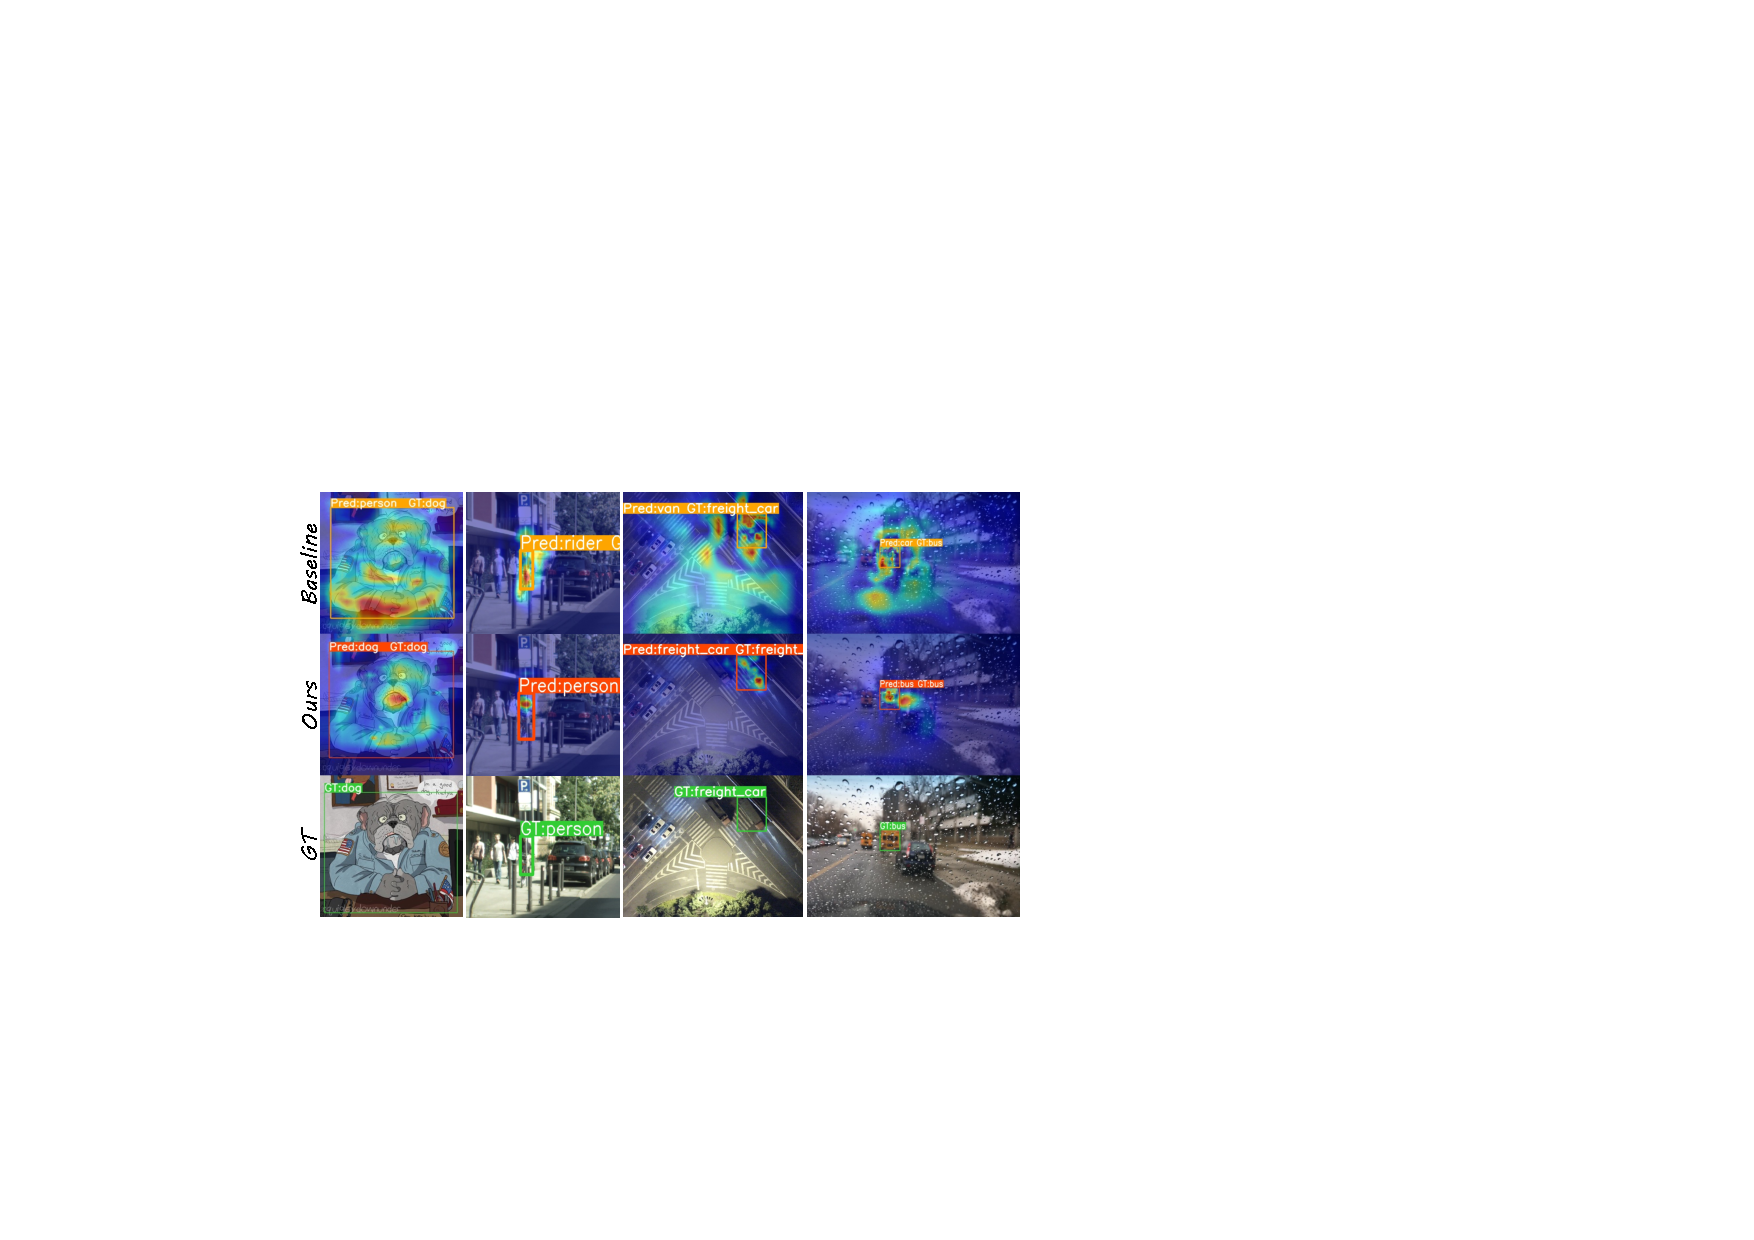
\includegraphics[width=0.44\textwidth]{figs/heatmap.pdf}
    \vspace{-3mm}
    \caption*{\textcolor{red}{Figure~A}. Visualization of the gradient responses of the detector.}
    \label{fig:heatmap}
\vspace{-3mm}
\end{figure}
\begin{table}[t!]
    \centering
    \caption*{\textcolor{red}{Table~B}. Average improvement (\%) of our method over DINOv2 and DINOv3 on FoggyCityscapes.}
    \vspace{-10pt}
    \label{tab:avg_improve}
    \footnotesize 
    \setlength{\tabcolsep}{3pt} 
    \begin{tabular}{lcccccccc}
    \toprule
    \textbf{Bus} & \textbf{Bike} & \textbf{Car} & \textbf{Motor} & \textbf{Psn.} & \textbf{Rider} & \textbf{Train} & \textbf{Truck} \\
    \midrule
    6.2\,$\uparrow$ & 6.4\,$\uparrow$ & 2.6\,$\uparrow$ & 4.1\,$\uparrow$ & 4.6\,$\uparrow$ & 3.2\,$\uparrow$ & 7.2\,$\uparrow$ & 2.9\,$\uparrow$ \\
    \bottomrule
    \end{tabular}
    \vspace{-16pt}
\end{table}
%may need to be removed due to space limit
% To further validate these observations, we conduct quantitative experiments to identify categories that are particularly susceptible to confounder effects.



\noindent\textbf{\textcolor{red}{aZkC}: Generalization.}
% We thank the reviewer for the suggestion and plan to include more comparison experiments in the revised version. 
\textit{Semantic Segmentation}: We evaluate our method on domain generalization for {semantic segmentation}, as shown in 
% Tab.~\ref{tab:segmentation_results}. 
\textcolor{red}{Table~C}.
Specifically, we train Mask2Former models with a frozen DINOv3 backbone on Cityscapes and evaluate them on BDD100K and Mapillary.
\begin{table}[ht]
\vspace{-16pt}
\centering
\footnotesize 
\caption*{\textcolor{red}{Table~C}. Cross-domain semantic segmentation: Cityscapes to BDD100K and Mapillary}
\vspace{-10pt}
% \setlength{\tabcolsep}{8pt} 
\begin{tabular}{lccc}
\toprule
\textbf{Method} & \textbf{BDD100K} & \textbf{Mapillary} & \textbf{Avg.} \\
\midrule
Baseline & 65.25 & 74.45 & 69.85 \\
Ours     & \textbf{65.77} & \textbf{75.78} & \textbf{70.78} \\
\bottomrule
\end{tabular}
\vspace{-12pt}
\label{tab:segmentation_results}
\end{table}



\noindent\textit{Classification.} On DomainBed, we use a frozen DINOv2 trained with the ERM strategy as the baseline and build our method by adapting the learnable basis projection strategy. Results ($56.8 \pm 0.6$~vs.~$\mathbf{58.2 \pm 0.6}$, training-domain-validation model selection strategy) on the TerraIn dataset demonstrate the generalizability beyond detection task.
% \noindent\textit{Classification.} Due to limited rebuttal time, we were unable to include the classification on DomainBed at this stage. We believe that our method's consistent performances on object detection and semantic segmentation across multiple datasets and backbones indicate a strong generalizability.




















%%%%%%%%% REFERENCES
% {
%     \small
%     \bibliographystyle{ieeenat_fullname}
%     \bibliography{main}
% }

\end{document}
